\chapter{Конструкторский раздел}

\section{Последовательность преобразований}

На рисунке \ref{img:idef0} приведена диаграмма состояний IDEF0 нулевого уровня, а на рисунке \ref{img:idef1} --- диаграмма состояний IDEF0 первого уровня.

\begin{figure}[H]
	\begin{center}
		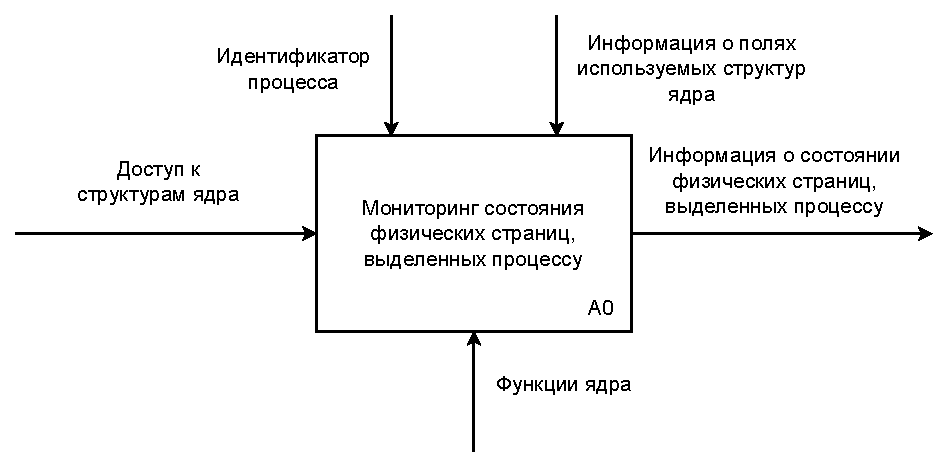
\includegraphics[scale=0.8]{inc/img/idef0.pdf}
	\end{center}
	\captionsetup{justification=centering}
	\caption{Диаграмма состояний IDEF0 нулевого уровня}
	\label{img:idef0}
\end{figure}

\begin{figure}[H]
	\begin{center}
		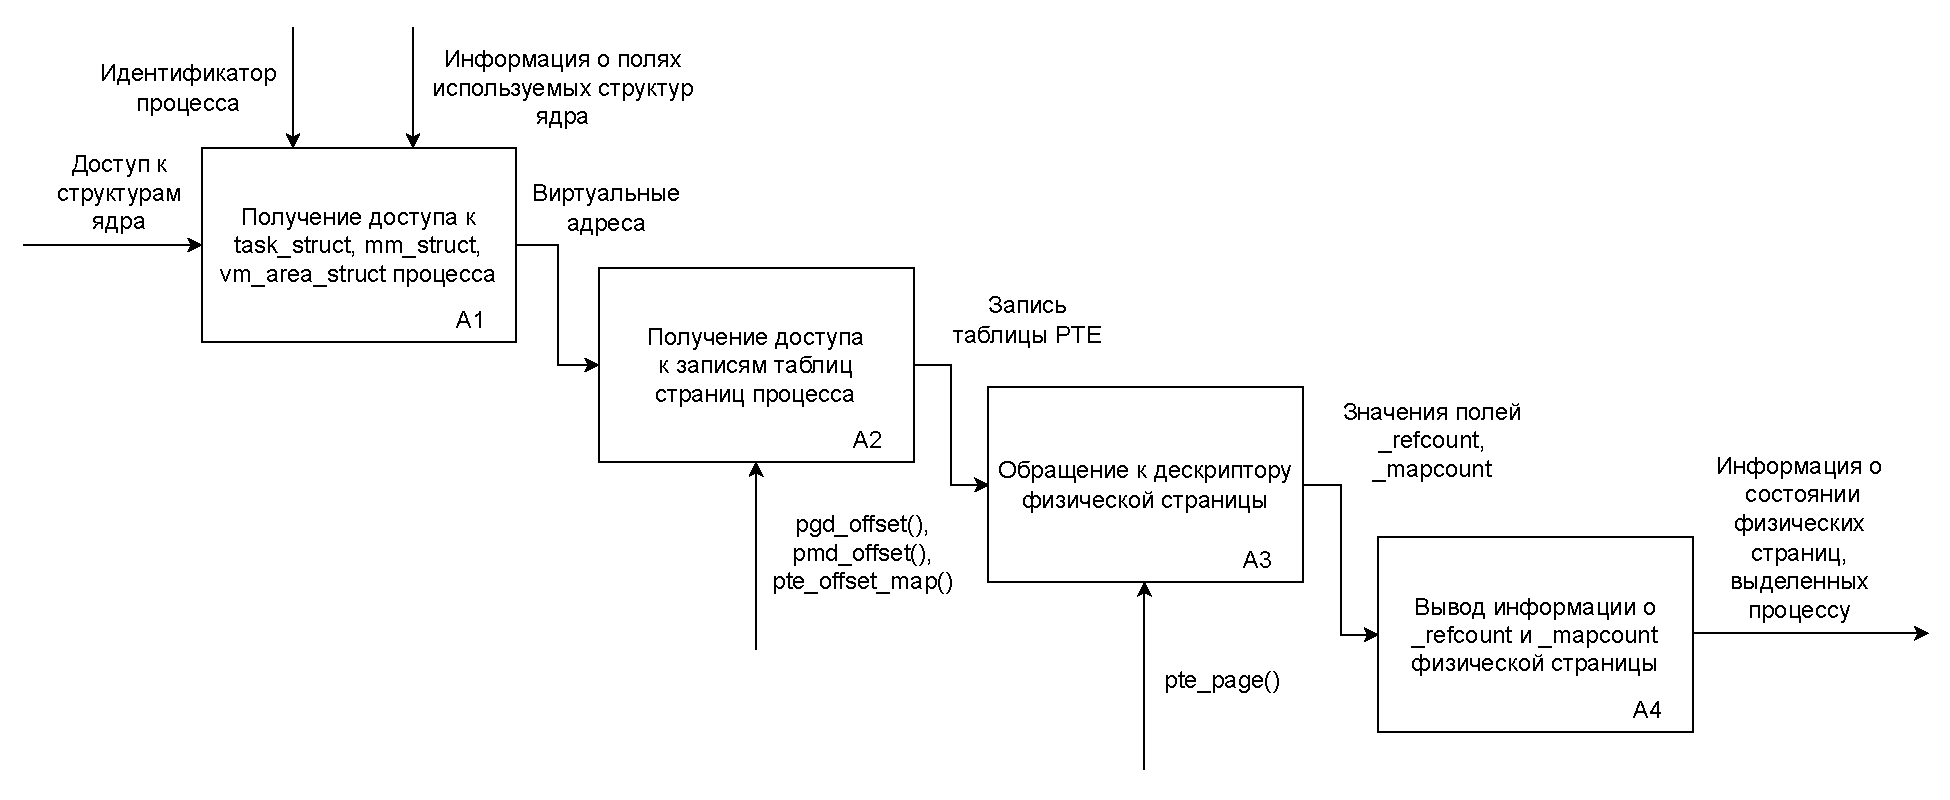
\includegraphics[scale=0.5]{inc/img/idef1.pdf}
	\end{center}
	\captionsetup{justification=centering}
	\caption{Диаграмма состояний IDEF0 первого уровня}
	\label{img:idef1}
\end{figure}

\section{Алгоритм сканирования виртуальных страниц}

На рисунке \ref{img:trace_pages} представлена схема алгоритма сканирования виртуальных страниц.

\begin{figure}[H]
	\begin{center}
		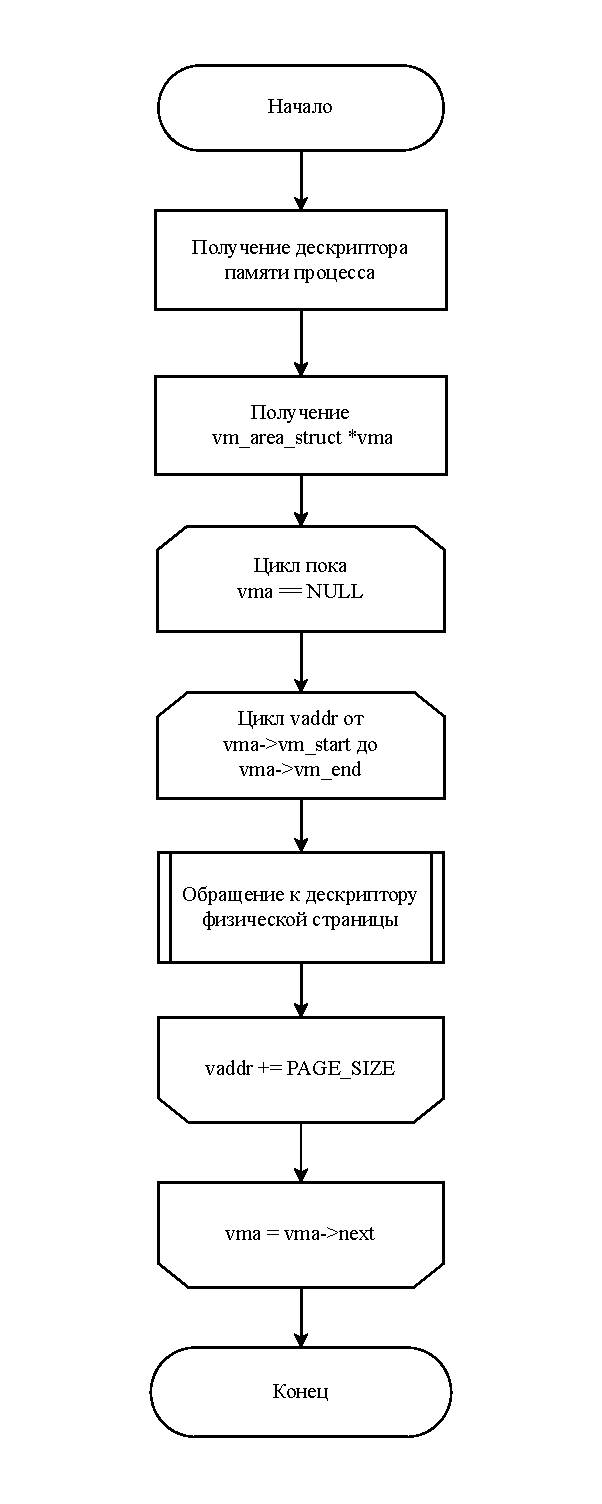
\includegraphics[scale=0.75]{inc/img/trace_pages.pdf}
	\end{center}
	\captionsetup{justification=centering}
	\caption{Алгоритм сканирования виртуальных страниц}
	\label{img:trace_pages}
\end{figure}

\section{Алгоритм обращения к дескриптору физической страницы}

На рисунке \ref{img:get-page} показана схема алгоритма обращения к дескриптору физической страницы.

\begin{figure}[H]
	\begin{center}
		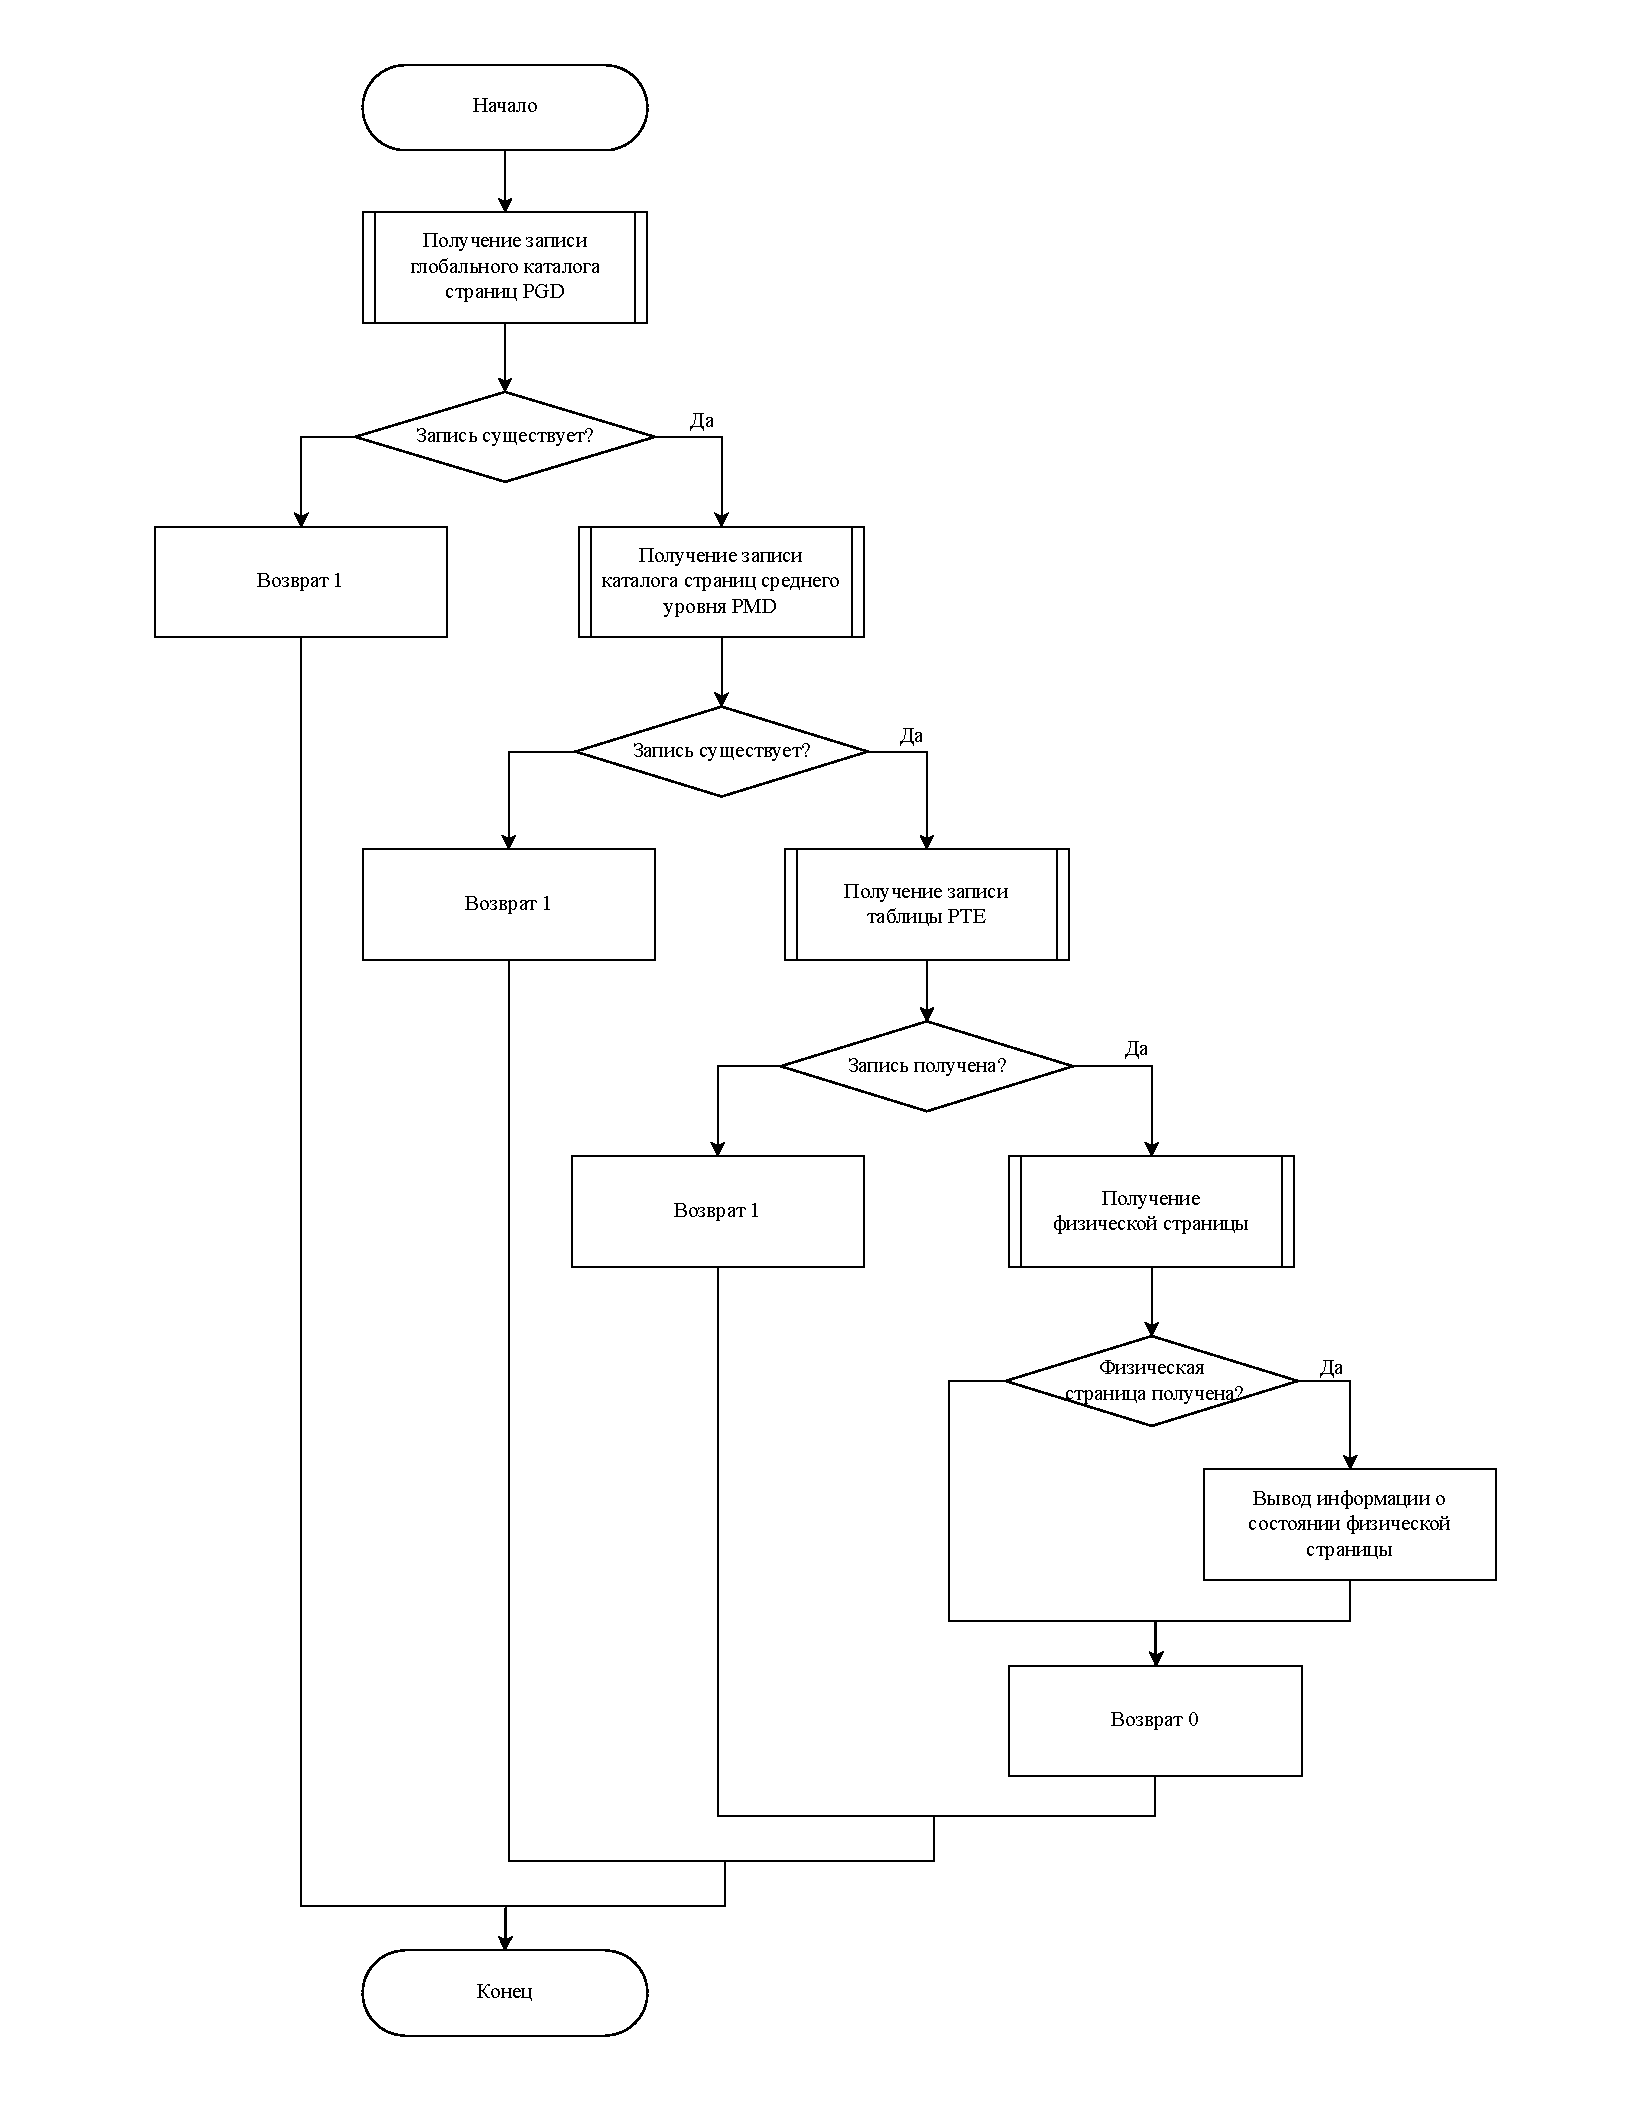
\includegraphics[scale=0.65]{inc/img/get_page.pdf}
	\end{center}
	\captionsetup{justification=centering}
	\caption{Алгоритм обращения к дескриптору физической страницы}
	\label{img:get-page}
\end{figure}

\section{Алгоритм получения информации о состоянии физической страницы}

На рисунке \ref{img:log-page} приведена схема алгоритма получения информации о состоянии физической страницы.

\begin{figure}[H]
	\begin{center}
		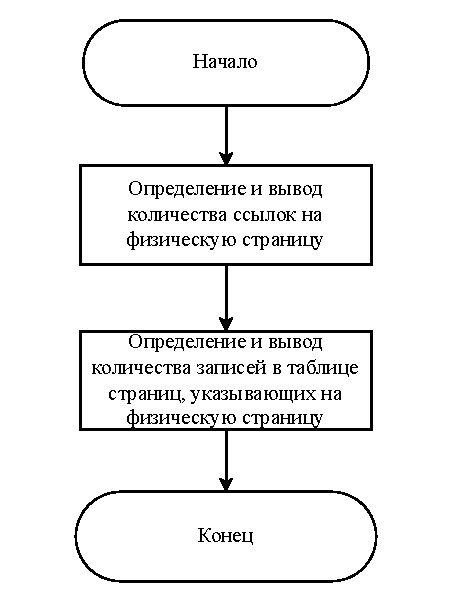
\includegraphics[scale=0.8]{inc/img/log_page.pdf}
	\end{center}
	\captionsetup{justification=centering}
	\caption{Алгоритм получения информации о состоянии физической страницы}
	\label{img:log-page}
\end{figure}

\section{Структура программного обеспечения}

На рисунке \ref{img:structure} представлена структура программного обеспечения.

\begin{figure}[H]
	\begin{center}
		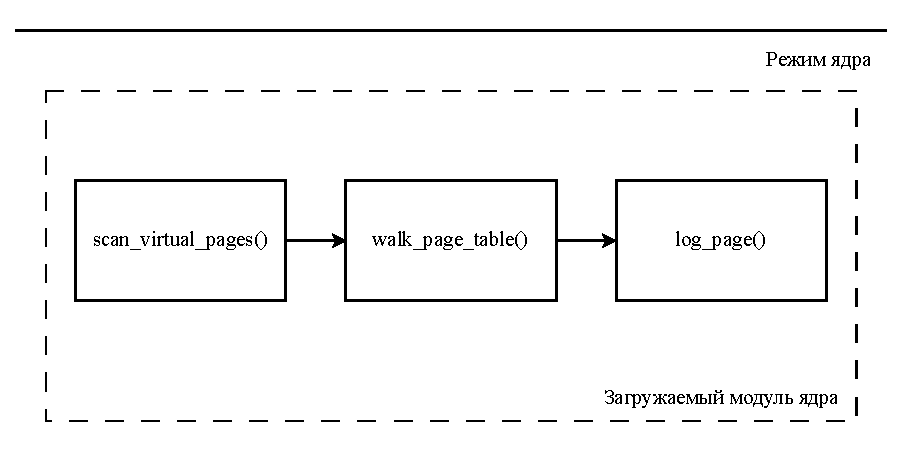
\includegraphics[scale=0.8]{inc/img/structure.pdf}
	\end{center}
	\captionsetup{justification=centering}
	\caption{Структура программного обеспечения}
	\label{img:structure}
\end{figure}
